\documentclass{article}

\usepackage{amsmath, amsthm, amssymb, amsfonts}
\usepackage{thmtools}
\usepackage{graphicx}
\usepackage{setspace}
\usepackage{geometry}
\usepackage{float}
\usepackage{hyperref}
\usepackage[utf8]{inputenc}
\usepackage[english]{babel}
\usepackage{framed}
\usepackage[dvipsnames]{xcolor}
\usepackage{tcolorbox}

\colorlet{LightGray}{White!90!Periwinkle}
\colorlet{LightOrange}{Orange!15}
\colorlet{LightGreen}{Green!15}

\newcommand{\HRule}[1]{\rule{\linewidth}{#1}}

\declaretheoremstyle[name=Theorem,]{thmsty}
\declaretheorem[style=thmsty,numberwithin=section]{theorem}
\tcolorboxenvironment{theorem}{colback=LightGray}

\declaretheoremstyle[name=Proposition,]{prosty}
\declaretheorem[style=prosty,numberlike=theorem]{proposition}
\tcolorboxenvironment{proposition}{colback=LightOrange}

\declaretheoremstyle[name=Principle,]{prcpsty}
\declaretheorem[style=prcpsty,numberlike=theorem]{principle}
\tcolorboxenvironment{principle}{colback=LightGreen}

\setstretch{1.2}
\geometry{
    textheight=9in,
    textwidth=5.5in,
    top=1in,
    headheight=12pt,
    headsep=25pt,
    footskip=30pt
}

% ------------------------------------------------------------------------------

\begin{document}

% ------------------------------------------------------------------------------
% Cover Page and ToC
% ------------------------------------------------------------------------------

\title{ \normalsize \textsc{}
		\\ [2.0cm]
		\HRule{1.5pt} \\
		\LARGE \textbf{\uppercase{Combinatorics Space/Time Complexity}
		\HRule{2.0pt} \\ [0.6cm] \LARGE{An analysis of the space/time complexity from resulting combinatorics graphs.} \vspace*{10\baselineskip}}
		}
\date{}
\author{\textbf{Author} \\ 
		Jack Carmichael \\
		  Andrew Burford \\
		4/19/2023}

\maketitle
\newpage

\tableofcontents
\newpage

% ------------------------------------------------------------------------------
\section{The Problem}
\label{sec:Problem}

The problem can be described from a simple scenario:
\begin{itemize}
    \item You have a set of items
    \item You want to perform the following operation starting with the full set of items:
    \begin{enumerate}
        \item Take one item from the set. Any item can be taken away so this will result in many possible outcomes for new sets.
        \item For each new set continue to take away one item.
        \item Do this until no items are left.
    \end{enumerate}
\end{itemize}

Given that scenario, the question is threefold:
\begin{enumerate}
    \item How many ways can the final empty set be reached?
    \item What is the time complexity of searching each path to reach the final empty set compared to the number of nodes?
    \item What is the space complexity of storing every path compared to the number of nodes?
\end{enumerate}

\section{Symbol Soup}
\label{sec:SymbolSoup}

This section is here for convenience to list all of the symbols that will be used. It can serve as a reference as you read the paper.

\begin{table}[h]
    \centering
    \begin{tabular}{|c|c|}
        \hline
        Symbol &  Meaning \\
        \hline
        $S$ & The initial set of items \\
        \hline
        $c$ & The total number of columns in either the graph or pascals triangle \\
        \hline
        $n_c$ & Number of nodes in column $c$, an arbitrary column \\
        \hline
        $n_t$ & Total number of nodes \\
        \hline
        $e_{n,c}$ & Number of edges coming from node $n$ in column $c$, an arbitrary node and column \\
        \hline
        $e_c$ & Number of edges in column $c$, an arbitrary column \\
        \hline
        $e_t$ & Total number of edges \\
        \hline
    \end{tabular}
    \caption{An exhaustive list of symbols that will be used in this paper.}
    \label{tab:symbolList}
\end{table}

\section{Graph Representation and Pascals Triangle}
\label{sec:GraphAndPascalsTriangle}

Before moving forward it is helpful to see the problem in the form of a graph. Figure \ref{fig:} shows an example graph with an initial set, $S$, with six items, $|S|=6$.

Several things should be immediately apparent:
\begin{enumerate}
    \item The graph is symmetrical
    \item The graph closes in on itself past halfway, rather than continuing to bifurcate as a tree would.
\end{enumerate}

Beyond the initial observations, equations to represent the number of nodes and edges are needed. Once it is realized that the number of nodes in each 'column' can be calculated from a combinatoric, the equation to find the number of nodes at each column is easily found, and is shown in equation \ref{eq:NodesInColumn}. Since combinatorics are involved, pascals triangle must also be involved. Given $|S|$ flight computers, the number of columns and number of nodes in each column can be found from row $|S|+1$ of pascals triangle.

\begin{equation}
    n_c(i)=\binom{|S|}{i}=\frac{|S|!}{(|S|-i)!i!}
    \label{eq:NodesInColumn}
\end{equation}
\centerline{where $i$ is a valid column index, $c\in \{ 0\le i\le |S|\}$}

Following that, the total number of nodes in the graph can be found using equation \ref{eq:TotalNumNodes}.

\begin{equation}
    n_t=\sum_{i=0}^{|S|}n_c(i)=\sum_{i=0}^{|S|-1}\binom{|S|}{i}=\sum_{i=0}^{|S|}\frac{|S|!}{(|S|-i)!i!}
    \label{eq:TotalNumNodes}
\end{equation}

Finding the total number of edges seems to be more tricky, but the solution is to count the number of edges coming out of each node in each column. Looking at the example from figure \ref{fig:}, a clear linear pattern should be apparent. This pattern can be represented using equation \ref{eq:EdgesPerNodePerColumn}.

\begin{equation}
    e_{n,c}(i)=|S|-i\\
    \label{eq:EdgesPerNodePerColumn}
\end{equation}
\centerline{where $i$ is a valid column index, $c\in \{ 0\le i\le |S|\}$}

Given this, the total number of edges in each column can be found using equation \ref{eq:EdgesPerColumn} and the total number of edges in the graph can be found using \ref{eq:TotalNumEdges}.

\begin{equation}
    e_c(i)=n_c(i)e_{n,c}(i)=\binom{|S|}{i}\left(|S|-i\right)=
    \frac{|S|!}{(|S|-i)!i!}\left(|S|-i\right)
    \label{eq:EdgesPerColumn}
\end{equation}
\begin{equation}
    e_t=\sum_{i=0}^{|S|}e_c(i)=
    \sum_{i=0}^{|S|}\binom{|S|}{i}\left(|S|-i\right)=
    \sum_{i=0}^{|S|}\frac{|S|!}{(|S|-i)!i!}\left(|S|-i\right)
    \label{eq:TotalNumEdges}
\end{equation}

Equations \ref{eq:TotalNumNodes} and \ref{eq:TotalNumEdges} are the important results that will be used to compare time and space complexity. Now that the problem has been framed in a more mathematical light, the questions originally posed can be translated to the following:

\begin{enumerate}
    \item TODO: rewrite first question
    \item Given that every edge is traversed once and only once, what is the time complexity of traversing the full graph when compared to the number of nodes as $|S|\to\infty$?
    \item Given that every edge takes equal amounts of memory, what is the space used when compared to the number of nodes as $|S|\to\infty$?
\end{enumerate}

Now that the questions are posed mathematically, it is easy to see that the last two questions are actually asking the same thing. These questions will be answered together in sections \ref{sec:LowerBound}-\ref{sec:TightBound}. The first question will be answered first, in section \ref{sec:ReachingTheEmptySet}.

\section{Reaching the Empty Set}
\label{sec:ReachingTheEmptySet}

TODO?? Im tempted to remove this section and its associated question... It might open a whole nother can of worms...

%Ignore this, its wrong
% \begin{equation}
%     \prod_{i=0}^{|S|} n_te_t
% \end{equation}

\section{Big-$\Omega$: A Lower Bound}
\label{sec:LowerBound}

The question is if the number of total number of edges grows faster or slower than the total number of nodes. In order for the total number of edges to grow slower than the total number of nodes the inequality shown in equation \ref{eq:nInequality} must be true.

\begin{equation}
    \begin{split}
        \forall i\in c\;\; \sum_{i=0}^{|S|}\frac{|S|!}{(|S|-i)!i!}(|S|-i) & \ge \sum_{i=0}^{|S|}\frac{|S|!}{(|S|-i)!i!}
    \end{split}
    \label{eq:nInequality}
\end{equation}

This is true given that $|S|-i\neq0$, which will only happen when $i=|S|$. However the difference in that scenario will only ever be $1$, which is easily overcome by all the other summation values. Not much need be explained here. This proves that the number of edges grows more than the number of nodes, or $e_t\in \Omega(n_t)$.

\section{Big-O: An Upper Bound}
\label{sec:UpperBound}

The question now is if the number of total number of edges grows faster or slower than the total number of nodes squared. In order for the total number of edges to grow slower than the total number of nodes squared the inequality shown in equation \ref{eq:nSquaredInequality} must be true.

\begin{equation}
    \begin{split}
        \forall i\in c\;\; \sum_{i=0}^{|S|}\frac{|S|!}{(|S|-i)!i!}(|S|-i) & \le \sum_{i=0}^{|S|}\left(\frac{|S|!}{(|S|-i)!i!}\right)^2
        \\
        \forall i\in c\;\; \sum_{i=0}^{|S|}\frac{|S|!}{(|S|-i)!i!}(|S|-i) & \le \sum_{i=0}^{|S|}\frac{|S|!}{(|S|-i)!i!}\sum_{j=0}^{|S|}\frac{|S|!}{(|S|-j)!j!}
    \end{split}
    \label{eq:nSquaredInequality}
\end{equation}

Looking at the last line in equation \ref{eq:nSquaredInequality}, it should be trivial to see that if equation \ref{eq:innerNSquaredInequality} is true then equation \ref{eq:nSquaredInequality} must also be true.

\begin{equation}
    \forall i\;\; f-i\le\sum_{i=0}^{|S|}\frac{|S|!}{(|S|-i)!i!}
    \label{eq:innerNSquaredInequality}
\end{equation}

The LHS of equation \ref{eq:innerNSquaredInequality} is greatest when $i=0$.\footnote{Note that the $i$ on the LHS of equation \ref{eq:innerNSquaredInequality} is different from the $i$ in the summation on the RHS which will always start at $0$.} Even when the LHS of the equation is at it's greatest, it should be trivial to see that the RHS will always be $\ge$ the LHS. Remembering that the RHS represents a combinatoric, another way to view the RHS is as the summation of all the columns in row $|S|+1$ in pascals triangle, which will always be $\ge|S|$. In even simpler terms, there will always be equal or more ways to make unique sets from an initial set than the number of items in the original set.

This proves that the number of edges grows less than the number of nodes squared, or $e_t\in O(n_t^2)$.

\section{Big $\Theta$: A Tight Bound}
\label{sec:TightBound}

The previous sections did not have to consider the effects as $|S|\to \infty$ because there results were trivially proven for all $i$, regardless of $|S|$. This section cannot afford that luxury, necessitating the more formal definition of time complexity. For this section, the inequalities shown in equation \ref{eq:nlognInequality} must be true.

\begin{equation}
    \begin{split}
        \forall n_t\ge n_o \;\; &
        c_1\sum_{i=0}^{|S|}\frac{|S|!}{(|S|-i)!i!}
        \log \left( \sum_{j=0}^{|S|-1}\frac{|S|!}{(|S|-j)!j!} \right)
        \le
        \sum_{i=0}^{|S|}\frac{|S|!}{(|S|-i)!i!}(|S|-i)
        \\
        \forall n_t\ge n_o \;\; &
        \sum_{i=0}^{|S|}\frac{|S|!}{(|S|-i)!i!}(|S|-i)
        \le
        c_2\sum_{i=0}^{|S|}\frac{|S|!}{(|S|-i)!i!}
        \log \left( \sum_{j=0}^{|S|}\frac{|S|!}{(|S|-j)!j!} \right)
    \end{split}
    \label{eq:nlognInequality}
\end{equation}

The mathematical notation is getting a bit dense, so a leap in logic is required. Representing the number of nodes and edges with summations makes performing mathematical operations difficult. A more standard equation for the total number of nodes and edges is required.

Going all the way back to the original problem definition, another way to think about the nodes is as the set of all possible combinations from the original set, and it turns out this idea already has a name. The nodes represent the power set of the original set, or $P(S)$, meaning the number of nodes is equal to the size of the power set, or $n_t=|P(S)|$. All that's needed is the formula for the power set and a new equation to represent $n_t$ has been found. This is shown in equation \ref{eq:TotalNumNodesPowerSet}.

\begin{equation}
    n_t=|P(S)|=2^{|S|}
    \label{eq:TotalNumNodesPowerSet}
\end{equation}

The equation for the total number of edges requires more thought. For the total number of edges it helps to write out the terms from an example with a small value for $|S|$. It can be observed that the terms repeat themselves which allows for a simplification where half of the terms can just be multiplied by two. This result makes intuitive sense because the graph in figure \ref{fig:} is symmetrical.

\begin{equation*}
    \begin{split}
        \sum_{i=0}^{4-1}\frac{4!}{(4-i)!i!}(4-i)&=
        \sum_{i=0}^{4-1}\frac{4!}{(4-i-1)!i!}
        \\
        &=
        \left(\frac{4!}{3!0!}\right)
        \left(\frac{4!}{2!1!}\right)
        \left(\frac{4!}{1!2!}\right)
        \left(\frac{4!}{0!3!}\right)
        \\
        &=
        2
        \left(\frac{4!}{3!0!}\right)
        \left(\frac{4!}{2!1!}\right)
    \end{split}
\end{equation*}

Given the simplifications shown above, equation \ref{eq:edgesSymmetry} must also be true.

\begin{equation}
    \sum_{i=0}^{\frac{|S|}{2}}\frac{|S|!}{(|S|-i)!i!}\left(|S|-i\right)=
    \sum_{i=\frac{|S|}{2}}^{|S|}\frac{|S|!}{(|S|-i)!i!}\left(|S|-i\right)
    \label{eq:edgesSymmetry}
\end{equation}

Given that equation \ref{eq:edgesSymmetry} is true, the following sequence of simplifications can be made to equation \ref{eq:TotalNumEdges}.

\begin{equation*}
    \begin{split}
        e_t=\sum_{i=0}^{|S|}\frac{|S|!}{(|S|-i)!i!}\left(|S|-i\right)&=
        \sum_{i=0}^{\frac{|S|}{2}}\frac{|S|!}{(|S|-i)!i!}\left(|S|-i\right)+
        \sum_{i=\frac{|S|}{2}}^{|S|}\frac{|S|!}{(|S|-i)!i!}\left(|S|-i\right)
        \\
        &=
        \sum_{i=0}^{\frac{|S|}{2}}\frac{|S|!}{(|S|-i)!i!}\left(|S|-i\right)+
        \sum_{i=0}^{\frac{|S|}{2}}\frac{|S|!}{(|S|-i)!i!}\left(i\right)
        \\
        &=
        \sum_{i=0}^{\frac{|S|}{2}}\frac{|S|!}{(|S|-i)!i!}\left(|S|\right)
        \\
        &=
        \frac{|S|}{2}\sum_{i=0}^{|S|}\frac{|S|!}{(|S|-i)!i!}
        \\
        &=
        \frac{|S|}{2}n_t
    \end{split}
\end{equation*}

Looking at the final equation listed above it may be tempting to say that $e_t$ grows linearly with respect to $n_t$. This cannot be true however, because there is a relationship between $|S|$ and $n_t$: $n_t$ grows with increases in $|S|$. To make further progress, $|S|$ needs to be put in terms of $n_t$. This is possible with equation \ref{eq:TotalNumNodesPowerSet}, and the result is shown in equation \ref{eq:etInTermsOfNt}.

\begin{equation}
    \begin{split}
        \log(n_t)=|S|\log(2) \\
        e_t=\frac{1}{2\log(2)}n_t\log(n_t)
    \end{split}
    \label{eq:etInTermsOfNt}
\end{equation}

Using the final equation listed in equation \ref{eq:etInTermsOfNt} the inequalities listed in equation \ref{eq:nlognInequality} can be simplified to the inequalities shown in equation \ref{eq:nlognInequalitySimplified}.

\begin{equation}
    \begin{split}
        \forall n_t\ge n_o \;\; &
        c_1 n_t \log n_t \le \frac{1}{2\log(2)}n_t\log(n_t)
        \\
        \forall n_t\ge n_o \;\; &
        \frac{1}{2\log(2)}n_t\log(n_t) \le c_2 n_t \log n_t
    \end{split}
    \label{eq:nlognInequalitySimplified}
\end{equation}

The constants $c_1$ and $c_2$ can now easily be solved for.

\begin{equation}
    \begin{split}
        c_1 &\le \frac{1}{2\log(2)}
        \\
        c_2 &\ge \frac{1}{2\log(2)}
    \end{split}
\end{equation}

Given the inequalities for the constants, this proves that the number of edges grows with the number of nodes times the log of the number of nodes, or $e_t\in \Theta(n_t\log(n_t))$.

\section{Deeper Intuitions}
\label{sec:DeeperIntuitions}

TODO

\section{Examples}

\begin{theorem}
    This is a theorem.
\end{theorem}

\begin{proposition}
    This is a proposition.
\end{proposition}

\begin{principle}
    This is a principle.
\end{principle}

% Maybe I need to add one more part: Examples.
% Set style and colour later.

\subsection{Pictures}

\begin{figure}[htbp]
    \center
    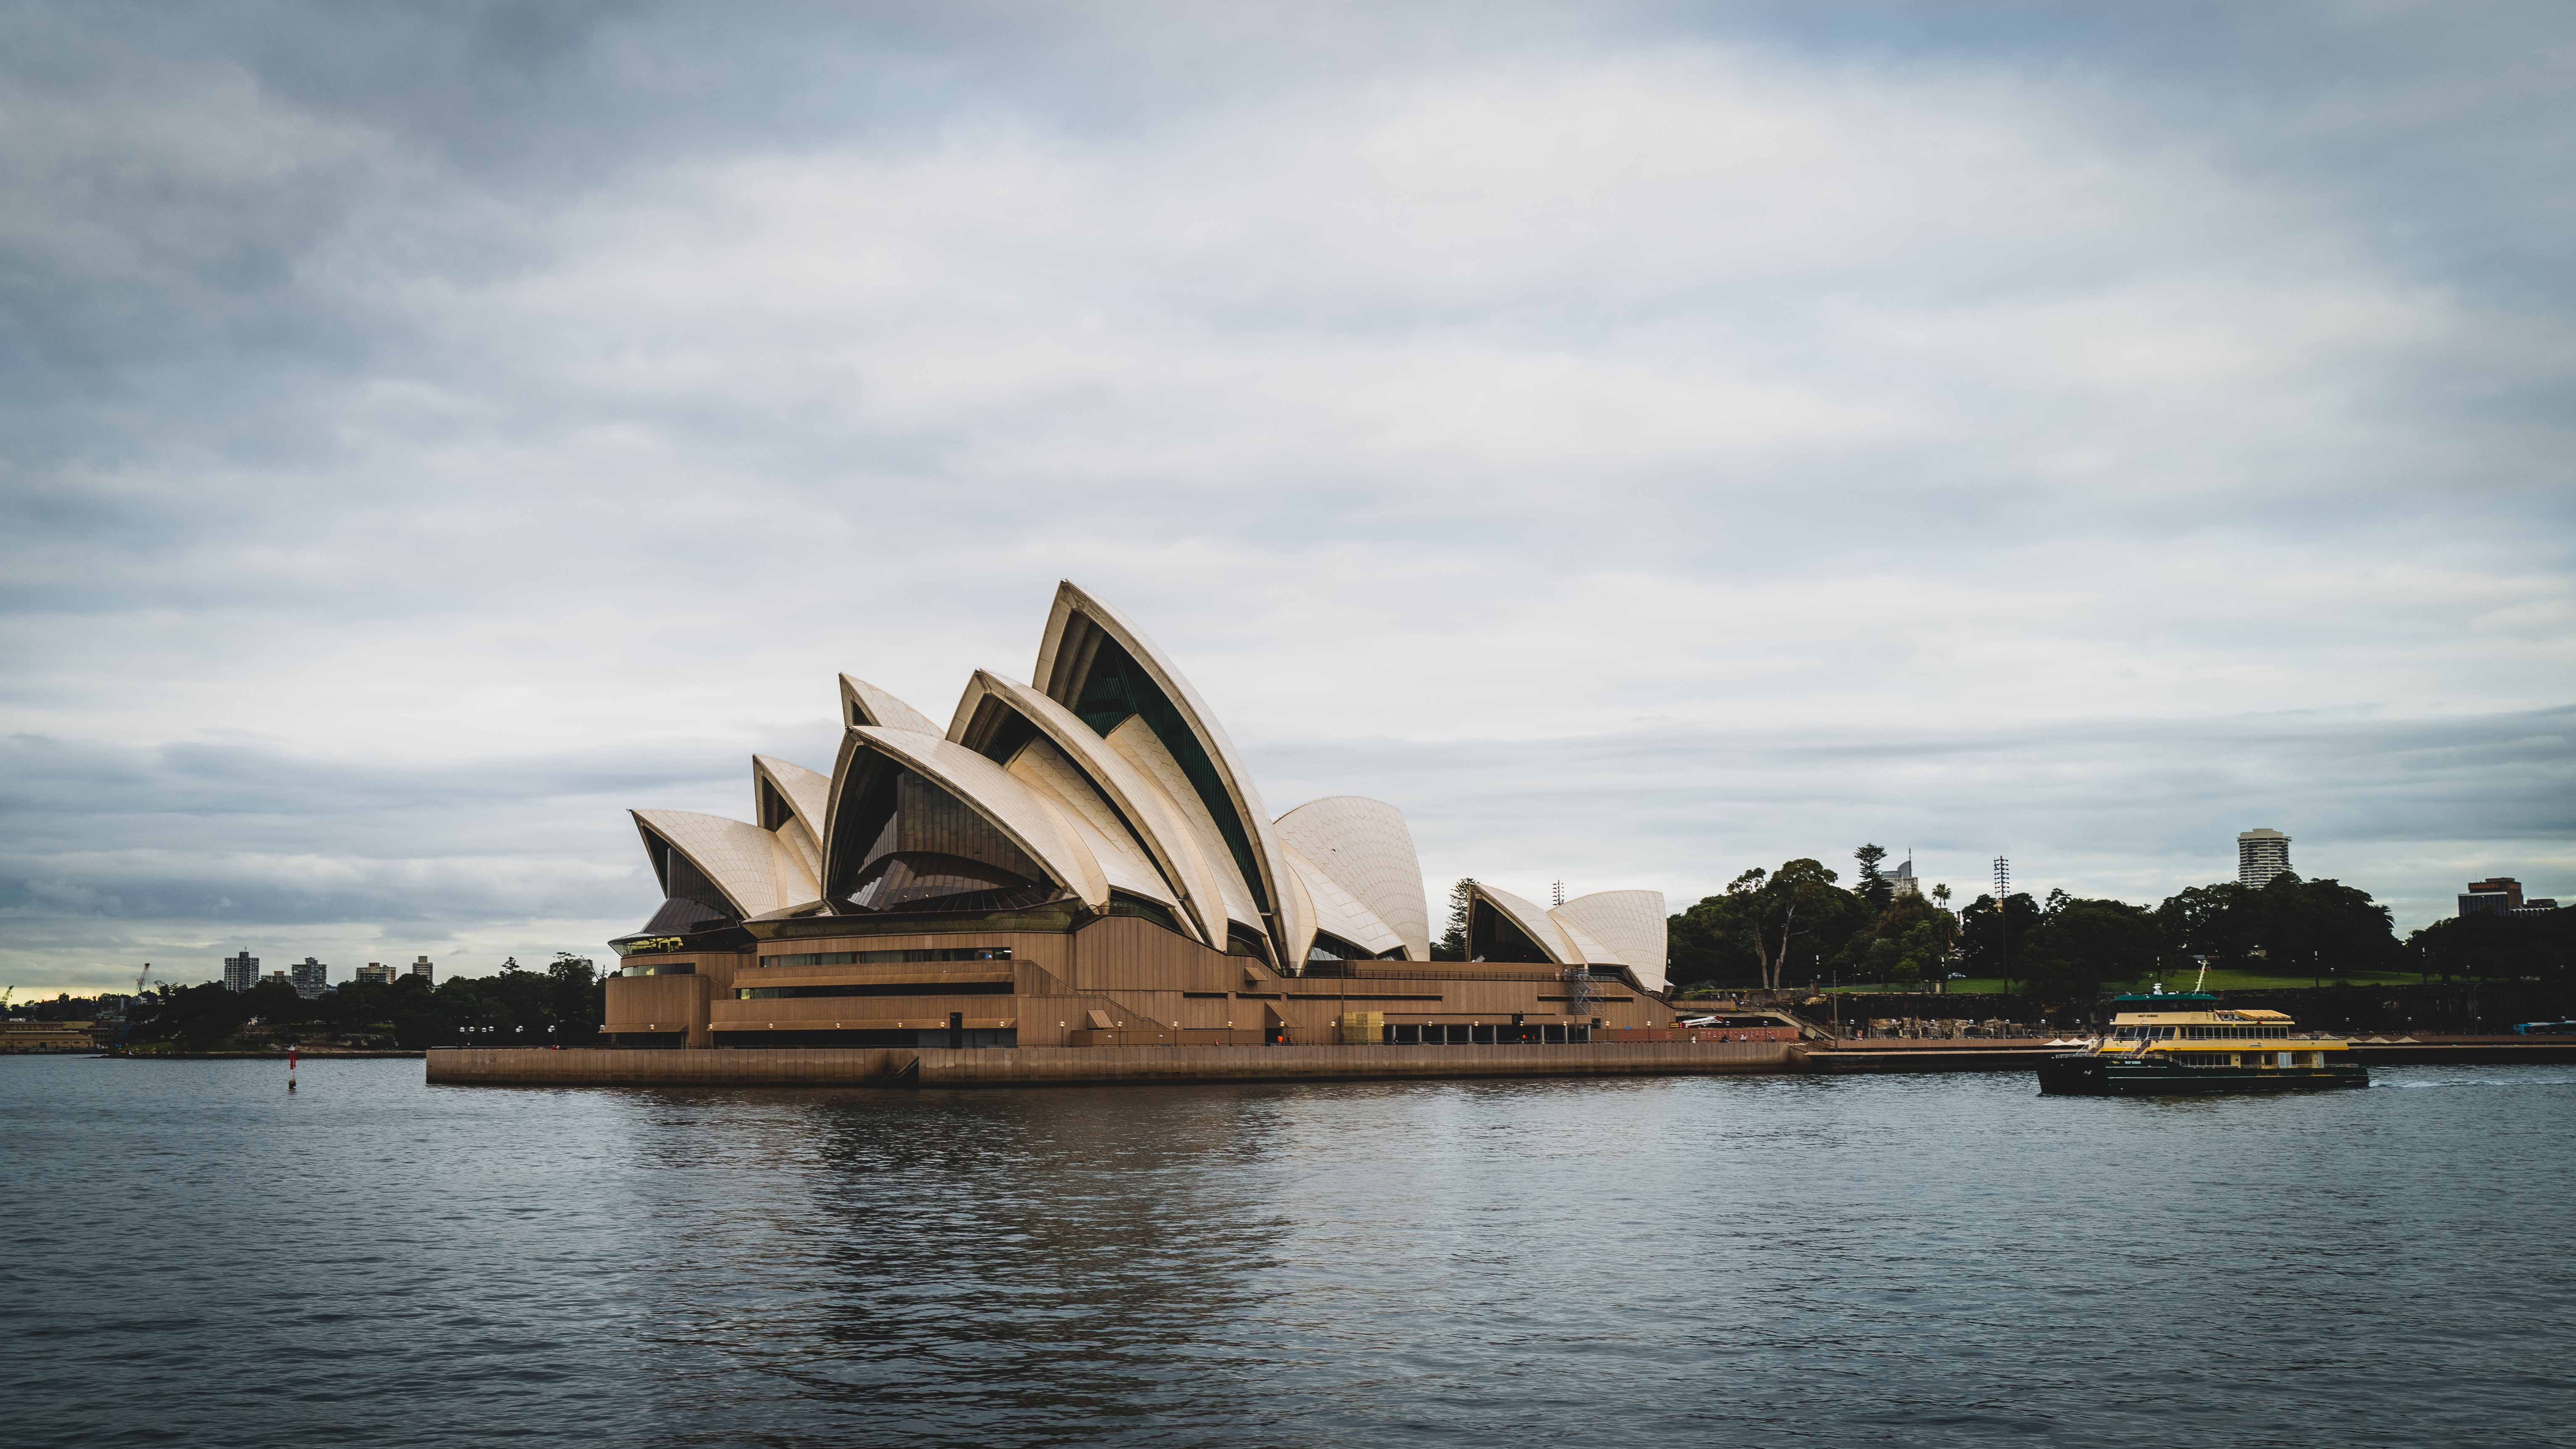
\includegraphics[scale=0.06]{img/photo.jpg}
    \caption{Sydney, NSW}
\end{figure}

\subsection{Citation}

This is a citation\cite{Eg}.

\newpage

% ------------------------------------------------------------------------------
% Reference and Cited Works
% ------------------------------------------------------------------------------

\bibliographystyle{IEEEtran}
\bibliography{References.bib}

% ------------------------------------------------------------------------------

\end{document}
